\documentclass[12pt, letterpaper]{article}


\usepackage{amsfonts,amssymb,latexsym}
\usepackage{amsthm}
\usepackage[margin=1in]{geometry}
\usepackage{graphicx}
\usepackage{amsmath}
\usepackage[font=footnotesize,labelfont=bf]{caption}
\usepackage{subfig}
\usepackage{placeins}
\usepackage{tikz}
\usetikzlibrary{calc,intersections}
\usepackage{bbm}
\usepackage{tikz}
\usetikzlibrary{arrows,automata}
\usetikzlibrary{positioning,calc}



\newcommand{\N}{\mathbb{N}}
\newcommand{\Z}{\mathbb{Z}}
\newcommand{\Q}{\mathbb{Q}}
\newcommand{\R}{\mathbb{R}}
\newcommand{\C}{\mathbb{C}}
\newcommand{\A}{\mathbb{A}}
\newcommand{\V}{\mathcal{V}}
\newcommand{\I}{\mathcal{I}}
\renewcommand{\P}{\mathbb{P}}
\newcommand{\G}{\mathbb{G}}
\newcommand{\F}{\mathbb{F}}
\newcommand{\B}{\mathbb{B}}
\newcommand{\T}{\mathbb{T}}
\newcommand{\M}{\frak{M}}
\newcommand{\D}{\mathcal{D}}
\renewcommand{\b}{\frak{b}}
\newcommand{\E}{\mathbb{E}}
%   ALGEBRA   %
\newcommand{\diag}{\ensuremath{\operatorname{diag}}}
\newcommand{\Span}{\ensuremath{\operatorname{Span}}}
\newcommand{\codim}{\ensuremath{\operatorname{codim}}}
\newcommand{\Spec}{\ensuremath{\operatorname{Spec}}}
\newcommand{\rad}{\ensuremath{\operatorname{rad}}}
\newcommand{\norm}{\mathrel{\lhd}}
\newcommand{\im}{\ensuremath{\operatorname{im}}}
\newcommand{\coker}{\ensuremath{\operatorname{coker}}}
\newcommand{\rank}{\ensuremath{\operatorname{rank}}}
\renewcommand{\char}{\ensuremath{\operatorname{char}}}
\newcommand{\Aut}{\ensuremath{\operatorname{Aut}}}
\newcommand{\la}{\langle}
\newcommand{\ra}{\rangle}
\newcommand{\orb}{\mathcal{O}}
\newcommand{\obj}{\ensuremath{\operatorname{obj}}}
\newcommand*\cat[1]{{\tt #1}}
\newcommand{\End}{\ensuremath{\operatorname{End}}}
\newcommand{\Hom}{\ensuremath{\operatorname{Hom}}}
\newcommand{\Ext}{\ensuremath{\operatorname{Ext}}}
\newcommand{\Tor}{\ensuremath{\operatorname{Tor}}}
\newcommand{\depth}{\ensuremath{\operatorname{depth}}}
\newcommand{\gldim}{\ensuremath{\operatorname{gldim}}}
\newcommand{\pd}{\ensuremath{\operatorname{pd}}}
\newcommand{\Kdim}{\ensuremath{\operatorname{Kdim}}}
\newcommand{\Flag}{\ensuremath{\operatorname{Flag}}}
\newcommand{\Stab}{\ensuremath{\operatorname{Stab}}}
\newcommand{\tr}{\ensuremath{\operatorname{tr}}}
\newcommand{\ch}{\ensuremath{\operatorname{ch}}}
\newcommand{\Sym}{\ensuremath{\operatorname{Sym}}}
\newcommand{\Irr}{\ensuremath{\operatorname{Irr}}}

%  LIE THEORY  %
\newcommand{\g}{\frak{g}}
\newcommand{\h}{\frak{h}}
\newcommand{\Ad}{\ensuremath{\operatorname{Ad}}}
\newcommand{\ad}{\ensuremath{\operatorname{ad}}}
\newcommand{\Der}{\ensuremath{\operatorname{Der}}}
\newcommand{\Lie}{\ensuremath{\operatorname{Lie}}}
\newcommand{\U}{\mathcal{U}}
\newcommand{\gl}{\frak{gl}}
\renewcommand{\sl}{\frak{sl}}
\newcommand{\Dist}{\ensuremath{\operatorname{Dist}}}


\newtheorem{thm}{Theorem}[section]
\newtheorem{prop}[thm]{Proposition}
\newtheorem{definition}{Definition}
\newtheorem*{thm1}{Theorem}
\newtheorem*{claim}{Claim}
\newtheorem{lem}[thm]{Lemma}
\newtheorem*{defn}{Definition}
\newtheorem{cor}[thm]{Corollary}
\newtheorem{conj}[thm]{Conjecture}
\newtheorem*{rem}{Remark}
  \let\oldrem\rem
  \renewcommand{\rem}{\oldrem\normalfont}
\newtheorem*{question}{Question}
\newtheorem{ex}[thm]{Example}
  \let\oldex\ex
  \renewcommand{\ex}{\oldex\normalfont}

\newcommand*\circled[1]{\tikz[baseline=(char.base)]{
            \node[shape=circle,draw,inner sep=2pt] (char) {#1};}}

%-------------------------------------------------------------------------------------------------------------------------------------------------------------------------------------




\title{Turing Machines and the Halting Problem}
\date{July 22, 2022}
\author{Nicholas Silva Tee}

\begin{document}
\maketitle
\begin{abstract}
A Turing machine is a mathematical model of computation and is represented as an abstract machine. As a part of Automata theory, a popular subject taught in undergraduate computer science departments. Turing machines are the most powerful of the different automata and have different versions, such as multi-tape and non-deterministic Turing machines. Coined by computer scientist Alan Turing, the halting problem is a popular decision problem considered to be unsolvable using Turing machines.
\end{abstract}

\section{Introduction}
This paper will review some fundamentals of automata theory before delving into Turing machines and their different variations. These variations include multi-tape and non-deterministic Turing machines. Other theoretical aspects of Turing machines will also be discussed, such as the Universal Turing machine. We will also cover the halting problem, it's proof of undecidability and applications of both the problem itself and Turing machines.




\subsection{History}
The initial intention of Turing was to recreate some of the "mechanical" processes we do as human beings. A paper was published titled "On Computable Numbers with an application to the Entscheidungsproblem" by Alan Turing himself in 1936. Entscheidungsproblem is the German word for "decision problem".\cite{brod} Turing suggested a universal machine that would be able to solve any problem and could be operated by using simple instructions on a tape, this would later be known as the "Universal Turing Machine" which we will discuss later on in this paper. The machine he described was completely a theoretical concept instead of an actual physical machine. The term "Turing Machine" was only actually coined by another mathematician Alonzo Church during a review of the paper.




\newpage
\section{Automata Theory}
In order to properly understand Turing machines, we first need to understand some of the more basic concepts within automata theory. Computer scientists use automata theory in order to better describe and understand the behaviour of discrete systems through "machines". Some of these major machines are known as \textbf{finite-state machines}, \textbf{pushdown automata}, and Turing machines.\\

In automata theory, all the different types of machines have three characteristics in common:\\
\textbf{Inputs:} An arbitrary set of symbols $\{ x_1, x_2, x_3, ... , x_n \}$ such that $n$ is the number of symbols. We will see that this set is commonly referred to as the \textbf{alphabet} of the finite-state machine.\\
\textbf{Outputs:} A set of output symbols $\{ y_1, y_2, y_3, ..., y_m \}$ such that $m$ is the number of symbols.\\
\textbf{States:} A finite set, normally defined as $Q$, the definition of this set, depends on the type of machine we are using. These can be considered as the "steps" in the automata.



\subsection{Finite-State Machines}
Finite-state machines may be classified into three different types:\\
\textbf{Acceptors:} these machines give us a binary output. Essentially, they take in an arbitrary input, and either accept or reject it.\\
\textbf{Classifiers:} A more generalized version of accepters, where the output is not binary and there are an $n$ types of outputs.\\
\textbf{Transducers:} Given some arbitrary input, it will generate an output(not binary)\\
In this paper, we will solely focus on acceptor types of state machines.\\

There are many different ways to define a finite-state machine, but we shall use the general mathematical definition.
\begin{defn}
A deterministic finite state machine is a quintuple/5-tuple denoted as $(\Sigma, S, s_0, \delta, F)$ such that:\\
\begin{itemize}
\item $\Sigma$: Is the non-empty set of possible inputs, also known as the alphabet
\item $S$: A non-empty, finite set of states.
\item $s_0$: The starting state and an element of $S$
\item $\delta$: Known as the "state-transition function", it is a function that can be defined as $\delta: S \times \Sigma \rightarrow S$.
$F$: The set of final states, or also known as accept states. The set may be empty, and is a subset of $S$.
\end{itemize} \cite{Ben}

\end{defn}
Note that the definition above is mean for a \textbf{deterministic} finite-state machine. There are Deterministic finite automata(DFA) and non-deterministic finite automata(NFA). The only difference between the two is that for each state in a DFA, there is only one transition, whereas each state in a NFA, may have more than one.\\

\begin{ex}
As a simple example, let us construct a DFA such that it only accepts strings that begin with the letter 'a'. With this high level description we can define the 5 elements that make a DFA such that, $\Sigma = \{a, b\}$, $S = \{s_0, s_1, s_2\}$, and $F = \{ s_1 \}$. We can then represent $\delta$ with the following table.

\begin{table}[!h]
\centering
\begin{tabular}{l|lll}
  & $s_0$ & $s_1$ & $s_2$ \\ \hline
a & $s_1$ & $s_1$ & $s_2$ \\
b & $s_2$ & $s_1$ & $s_2$
\end{tabular}
\end{table}
The top row represents the three states we have, and the leftmost column are the possible inputs for each state, we can see that if our starting state is $s_0$ and the input it receives is 'a', then the machine will move onto $s_1$ and will stay there. DFA's are also commonly drawn out in a graphical notation.


\begin{center}
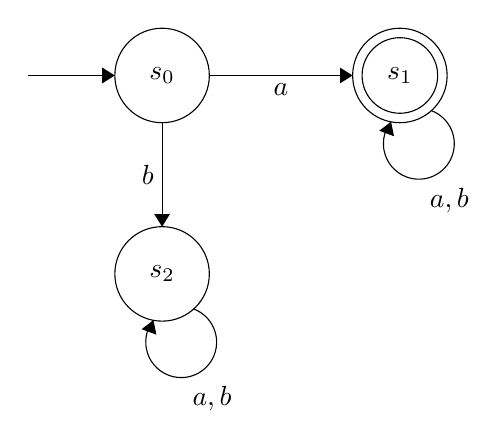
\begin{tikzpicture}[scale=0.2]
\tikzstyle{every node}+=[inner sep=0pt]
\draw [black] (16.3,-22) circle (3);
\draw (16.3,-22) node {$s_0$};
\draw [black] (31.4,-22) circle (3);
\draw (31.4,-22) node {$s_1$};
\draw [black] (31.4,-22) circle (2.4);
\draw [black] (16.3,-34.6) circle (3);
\draw (16.3,-34.6) node {$s_2$};
\draw [black] (19.3,-22) -- (28.4,-22);
\fill [black] (28.4,-22) -- (27.6,-21.5) -- (27.6,-22.5);
\draw (23.85,-22.5) node [below] {$a$};
\draw [black] (33.391,-24.228) arc (69.52411:-218.47589:2.25);
\draw (34.54,-29.1) node [below] {$a,b$};
\fill [black] (30.84,-24.94) -- (30.09,-25.51) -- (31.03,-25.86);
\draw [black] (16.3,-25) -- (16.3,-31.6);
\fill [black] (16.3,-31.6) -- (16.8,-30.8) -- (15.8,-30.8);
\draw (15.8,-28.3) node [left] {$b$};
\draw [black] (18.296,-36.824) arc (69.64225:-218.35775:2.25);
\draw (19.47,-41.7) node [below] {$a,b$};
\fill [black] (15.75,-37.54) -- (15,-38.11) -- (15.94,-38.46);
\draw [black] (7.8,-22) -- (13.3,-22);
\fill [black] (13.3,-22) -- (12.5,-21.5) -- (12.5,-22.5);
\end{tikzpicture}
\end{center}
The state which has a blank arrow pointing to it, in this case $s_0$ is how we draw the starting state. The state or states that have another circle drawn around it is how we represent a final state.
\end{ex}

Recall that NFA's are non-deterministic, so they have more than one possibility and will always lead into branching paths when processing an input.

\begin{ex}
Take the alphabet $\Sigma = \{ 0,1 \}$ and the language $L = \{ \text{all strings that end with 0} \}$. Constructing a DFA that accepts the language might be a little tricky, however, it is much easier when we use an NFA. We can simply use only 2 states to construct a machine that accepts the language, the transition table may be represented as:
\begin{table}[!h]
\centering
\begin{tabular}{l|ll}
  & $s_0$      & $s_1$ \\ \hline
1 & $s_0$      & $-$ \\
0 & $s_0, s_1$ & $-$
\end{tabular}
\end{table}
Notice how when $s_0$ reads a '0', it has two options, itself and $s_1$, this is where two branches are created and we must keep track of both. If any of the branches ends in a final state, then the NFA accepts the string. If no branch ends in a final state, it is rejected. A graphical drawing of this NFA may look like this:
\begin{center}
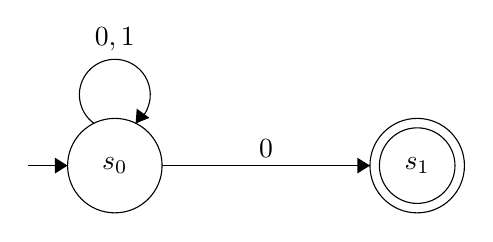
\begin{tikzpicture}[scale=0.2]
\tikzstyle{every node}+=[inner sep=0pt]
\draw [black] (5.7,-9) circle (3);
\draw (5.7,-9) node {$s_0$};
\draw [black] (24.9,-9) circle (3);
\draw (24.9,-9) node {$s_1$};
\draw [black] (24.9,-9) circle (2.4);
\draw [black] (8.7,-9) -- (21.9,-9);
\fill [black] (21.9,-9) -- (21.1,-8.5) -- (21.1,-9.5);
\draw (15.3,-8.5) node [above] {$0$};
\draw [black] (4.377,-6.32) arc (234:-54:2.25);
\draw (5.7,-1.75) node [above] {$0,1$};
\fill [black] (7.02,-6.32) -- (7.9,-5.97) -- (7.09,-5.38);
\draw [black] (0.2,-9) -- (2.7,-9);
\fill [black] (2.7,-9) -- (1.9,-8.5) -- (1.9,-9.5);
\end{tikzpicture}
\end{center}
For instance, let use '10' as an input. The first step is straightforward as it loops back to $s_0$. However, once '0' is read, we have two branches, one branch moves onto $s_1$ whilst the other stays in $s_0$. Since, one of the branches ends in a final state, the NFA accepts the string.\\

Similarly, if we take '01' as an input, we have our initial branch. However, since the next character in the input is '1', the branch that stayed in $s_0$ still stays there, and thus fails. The branch that moves onto $s_1$ does not have a transition, and thus automatically fails as well. Thus, the NFA does not accept the string.
\end{ex}

\begin{thm}
Every NFA can be reconstructed into an equivalent DFA
\end{thm}

NFA's also allow for \textbf{empty string} transitions. Represented by the $\epsilon$ symbol, it essentially acts as a free move within the transition function. Although they can technically be used in a DFA, they are more commonly found when designing NFA's.

\subsection{Pushdown Automata}
Similar to a DFA, pushdown automata (PDA) have the same characteristics, but also add two more:\\
$\Gamma$: The set of pushdown symbols, essentially a stack.\\
$Z$: The initial symbol we push into the stack.\\
\begin{rem}
In computer science, a stack is a way of storing information, where you can only look at the most recent thing stored (the top of the stack). An analogy for understanding this concept is by thinking of a stack of plates, where you can only "access" the top plate, where you can remove it, or add another plate on top. When \textbf{push} onto the stack when we add a symbol, and \textbf{pop} when we remove symbols. If the PDA has gone through the entire input, and $Z$ has been popped off the stack, then we accept the input.
\end{rem}
\begin{ex}
Given that $\Sigma = \{ a, b \}$ and the language $L = \{ a^nb^n | n \geq 0, n \in \N \}$ (Strings such as 'ab', 'aabb' and 'aaabbb'), lets design our PDA. We have $S = \{ s_0, s_1, s_2, s_3 \}$ and $F = \{ s_0, s_3 \}$. Since PDA's are more complicated than DFA's, lets start with a high level description of the process:
\begin{enumerate}
\item push $Z$ onto the stack
\item if we read an 'a' in the input, push 'a' onto the stack. If we see 'b' while pushing, we halt. else, we move to (step 3)
\item if we read 'b', we pop 'a'. If we still read 'b' and there is no 'a' left in the stack, we halt.
\item Pop $Z$ and accept the strin
\end{enumerate}

We can draw out the PDA in graphical notation, similar to what we did with the DFA, but instead the transitions are formatted as such
\[ x, y \rightarrow z \]
Where $x$ is the input symbol being read, $y$ is the symbol being popped from the stack, and $z$ is the symbol being pushed. If we do not want to push or pop onto the stack, we can use $\epsilon$.
\begin{center}
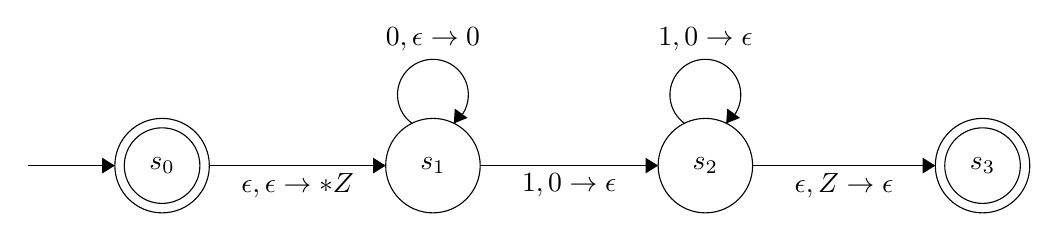
\begin{tikzpicture}[scale=0.2]
\tikzstyle{every node}+=[inner sep=0pt]
\draw [black] (14.2,-22) circle (3);
\draw (14.2,-22) node {$s_0$};
\draw [black] (14.2,-22) circle (2.4);
\draw [black] (31.4,-22) circle (3);
\draw (31.4,-22) node {$s_1$};
\draw [black] (48.7,-22) circle (3);
\draw (48.7,-22) node {$s_2$};
\draw [black] (66.3,-22) circle (3);
\draw (66.3,-22) node {$s_3$};
\draw [black] (66.3,-22) circle (2.4);
\draw [black] (5.7,-22) -- (11.2,-22);
\fill [black] (11.2,-22) -- (10.4,-21.5) -- (10.4,-22.5);
\draw [black] (17.2,-22) -- (28.4,-22);
\fill [black] (28.4,-22) -- (27.6,-21.5) -- (27.6,-22.5);
\draw (22.8,-22.5) node [below] {$\epsilon,\epsilon\rightarrow *Z$};
\draw [black] (34.4,-22) -- (45.7,-22);
\fill [black] (45.7,-22) -- (44.9,-21.5) -- (44.9,-22.5);
\draw (40.05,-22.5) node [below] {$1,0\rightarrow\epsilon$};
\draw [black] (51.7,-22) -- (63.3,-22);
\fill [black] (63.3,-22) -- (62.5,-21.5) -- (62.5,-22.5);
\draw (57.5,-22.5) node [below] {$\epsilon,Z\rightarrow\epsilon$};
\draw [black] (30.077,-19.32) arc (234:-54:2.25);
\draw (31.4,-14.75) node [above] {$0,\epsilon\rightarrow0$};
\fill [black] (32.72,-19.32) -- (33.6,-18.97) -- (32.79,-18.38);
\draw [black] (47.377,-19.32) arc (234:-54:2.25);
\draw (48.7,-14.75) node [above] {$1,0\rightarrow\epsilon$};
\fill [black] (50.02,-19.32) -- (50.9,-18.97) -- (50.09,-18.38);
\end{tikzpicture}
\end{center}


\end{ex}




\section{Turing Machines}



\subsection{Basics}



Turing machines can be thought of as more powerful versions of PDA's. First, instead of a stack, we now have an infinite tape to store our information, and we can only read and write to one digit on the tape at a time. A visualisation of this tape might look like this:
\begin{center}
\begin{figure}[h!]
	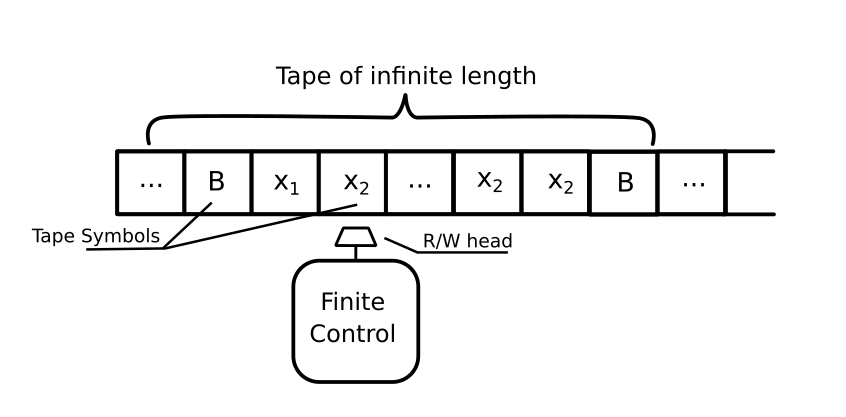
\includegraphics[scale=0.5]{tape.png}
\end{figure}
\end{center}
Turing machines have 4 main actions that it can do:
\begin{enumerate}
\item move right on the tape
\item move left on the tape
\item overwrite the current symbol on the tape with a new one
\item Halt and either accept the tape of reject.
\end{enumerate}

The output of the Turing machine will be the tape at the end of the process. Note that there is also the possibility that the Turing machine can be stuck in a loop and never halt, which will be discussed later on.\\

\begin{rem}
When scanning a Turing machine tape, the current section of the tape we are looking at is called the \textbf{tape head}
\end{rem}

\begin{defn}
We can define a Turing machine as a 7-tuple of $(Q, \Sigma, \Gamma, \delta, s_0, B, F)$ where:
\begin{itemize}
\item $Q$: non-empty set of states
\item $\Sigma$: alphabet / non-empty set of symbols used
\item $\Gamma$: non-empty set of tape symbols
\item $\delta$: The transition function defined as $Q \times \Sigma \rightarrow \Gamma \times (RL) \times Q$. Where $R$ and $L$ represent the right and left movement on the tape.
\item $s_0$: the initial state, $s_0 \in Q$
\item $B$: the blank symbol $\sqcup$, a special symbol to fill out the empty spaces on the infinite tape
\item $F$: Set of final states. However, in this case $F \not \subset Q$ as there are only two, 'ACCEPT' and 'REJECT'
\end{itemize}
\end{defn}
Furthermore, when creating the graph for a Turing machine, our transitions are formatted as such:
\[ x \rightarrow y, z \]
Where $x$ is the symbol currently being read on the tape, $y$ is the symbol we want to write onto the tape, and $z$ is the movement, whether we wish to move right or left. Similar to the PDA, if we do not wish to do any of these actions on a certain transition, we can always fill the spot with $\sqcup$.

\begin{ex}
Lets take the alphabet $\Sigma = \{ 1, 0, a, b \}$ and the language $L = \{ 01^n0 | n \geq 0 \}$. Ideally, it is quite simple to create a Turing machine that can accept this language, from a high-level perspective, the following steps can be taken:
\begin{enumerate}
\item Read the first symbol, if it is not a 0, then halt and reject, else move to step 2 and move tape right.
\item Keep reading 1's and moving right on the tape, if there is a blank, halt and reject. If a 0 is read, move to step 3
\item If a 1 or 0 is read, halt and reject, else, if a blank is read, halt and accept.
\end{enumerate}
The following Turing machine can then be drawing out as such:

\begin{center}
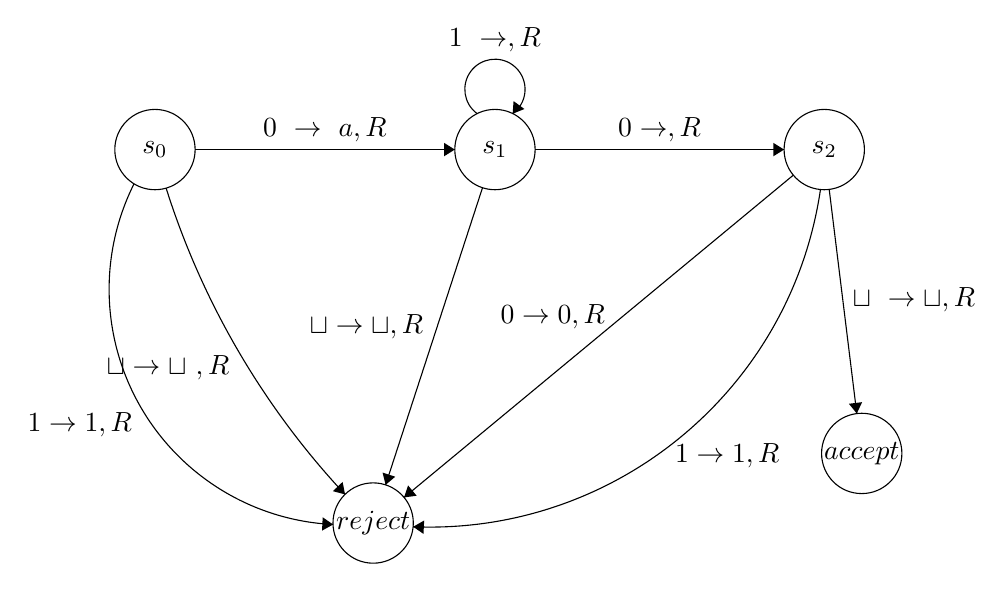
\begin{tikzpicture}[scale=0.17]
\tikzstyle{every node}+=[inner sep=0pt]
\draw [black] (9.4,-9.1) circle (3);
\draw (9.4,-9.1) node {$s_0$};
\draw [black] (34.8,-9.1) circle (3);
\draw (34.8,-9.1) node {$s_1$};
\draw [black] (59.4,-9.1) circle (3);
\draw (59.4,-9.1) node {$s_2$};
\draw [black] (62.2,-31.8) circle (3);
\draw (62.2,-31.8) node {$accept$};
\draw [black] (25.7,-37) circle (3);
\draw (25.7,-37) node {$reject$};
\draw [black] (12.4,-9.1) -- (31.8,-9.1);
\fill [black] (31.8,-9.1) -- (31,-8.6) -- (31,-9.6);
\draw (22.1,-8.6) node [above] {$0\mbox{ }\rightarrow\mbox{ }a,R$};
\draw [black] (33.477,-6.42) arc (234:-54:2.25);
\draw (34.8,-1.85) node [above] {$1\mbox{ }\rightarrow,R$};
\fill [black] (36.12,-6.42) -- (37,-6.07) -- (36.19,-5.48);
\draw [black] (37.8,-9.1) -- (56.4,-9.1);
\fill [black] (56.4,-9.1) -- (55.6,-8.6) -- (55.6,-9.6);
\draw (47.1,-8.6) node [above] {$0\rightarrow,R$};
\draw [black] (59.77,-12.08) -- (61.83,-28.82);
\fill [black] (61.83,-28.82) -- (62.23,-27.97) -- (61.24,-28.09);
\draw (61.47,-20.32) node [right] {$\sqcup\mbox{ }\rightarrow\sqcup,R$};
\draw [black] (22.706,-37.109) arc (-92.80874:-206.6018:17.595);
\fill [black] (22.71,-37.11) -- (21.93,-36.57) -- (21.88,-37.57);
\draw (7.72,-29.65) node [left] {$1\rightarrow1,R$};
\draw [black] (33.87,-11.95) -- (26.63,-34.15);
\fill [black] (26.63,-34.15) -- (27.35,-33.54) -- (26.4,-33.23);
\draw (29.48,-22.37) node [left] {$\sqcup\rightarrow\sqcup,R$};
\draw [black] (59.116,-12.085) arc (-8.35611:-92.40164:29.507);
\fill [black] (28.69,-37.28) -- (29.46,-37.81) -- (29.51,-36.81);
\draw (52.16,-31.02) node [below] {$1\rightarrow1,R$};
\draw [black] (23.598,-34.86) arc (-136.94667:-162.46388:59.989);
\fill [black] (23.6,-34.86) -- (23.42,-33.93) -- (22.69,-34.62);
\draw (14.99,-25.41) node [left] {$\sqcup\rightarrow\sqcup\mbox{ },R$};
\draw [black] (57.09,-11.01) -- (28.01,-35.09);
\fill [black] (28.01,-35.09) -- (28.95,-34.96) -- (28.31,-34.19);
\draw (39.12,-22.56) node [above] {$0\rightarrow0,R$};
\end{tikzpicture}
\end{center}
If we were to feed this Turing machine an input in L such as the string '0110'. The tape may look something like this.
\begin{center}
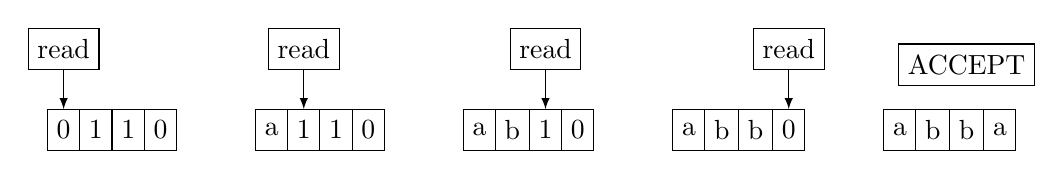
\begin{tikzpicture}[every node/.style={block},
        block/.style={minimum height=1.5em,outer sep=0pt,draw,rectangle,node distance=0pt}]
   \node (A) {1};
   \node (B) [left=of A] {1};
   \node (C) [left=of B] {0};
   \node (D) [right=of A] {0};
   \node (F) [above = 0.5cm of C] {read};
   \draw[-latex] (F) -- (C);
   
   \node (G) [right = 1 cm of D] {a};
   \node (H) [right=of G] {1};
   \node (I) [right=of H] {1};
   \node (J) [right=of I] {0};
   \node (K) [above = 0.5cm of H] {read};
   \draw[-latex] (K) -- (H);
   
   \node (L) [right = 1 cm of J] {a};
   \node (M) [right=of L] {b};
   \node (N) [right=of M] {1};
   \node (O) [right=of N] {0};
   \node (P) [above = 0.5cm of N] {read};
   \draw[-latex] (P) -- (N);
   
   \node (Q) [right = 1 cm of O] {a};
   \node (R) [right=of Q] {b};
   \node (S) [right=of R] {b};
   \node (T) [right=of S] {0};
   \node (U) [above = 0.5cm of T)] {read};
   \draw[-latex] (U) -- (T);
   
   \node (V) [right = 1 cm of T] {a};
   \node (X) [right=of V] {b};
   \node (Y) [right=of X] {b};
   \node (Z) [right=of Y] {a};
   \node (AA) [above = 0.3 cm of Y)] {ACCEPT};

\end{tikzpicture}
\end{center}
Note that the language can be accepted without having to overwrite the original symbols, but was done so in this example merely as a demonstration. Similarly, if we were to give the Turing machine an input of '0010', it would be rejected as such:

\begin{center}
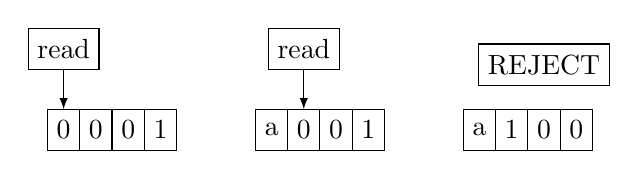
\begin{tikzpicture}[every node/.style={block},
        block/.style={minimum height=1.5em,outer sep=0pt,draw,rectangle,node distance=0pt}]
   \node (A) {0};
   \node (B) [left=of A] {0};
   \node (C) [left=of B] {0};
   \node (D) [right=of A] {1};
   \node (F) [above = 0.5cm of C] {read};
   \draw[-latex] (F) -- (C);
   
   \node (G) [right = 1 cm of D] {a};
   \node (H) [right=of G] {0};
   \node (I) [right=of H] {0};
   \node (J) [right=of I] {1};
   \node (K) [above = 0.5cm of H] {read};
   \draw[-latex] (K) -- (H);
      
   \node (V) [right = 1 cm of J] {a};
   \node (X) [right=of V] {1};
   \node (Y) [right=of X] {0};
   \node (Z) [right=of Y] {0};
   \node (AA) [above = 0.3 cm of Y)] {REJECT};

\end{tikzpicture}
\end{center}
\end{ex}
Recall that Turing machines do not necessarily have to halt and accept or reject, there is the possibility of a Turing machine never halting. With the alphabet $\Sigma = \{ 1,0 \}$, let us construct a Turing machine with the following rules.\\
\begin{itemize}
\item If a 1 is read on the tape, move right
\item If a 0 is read on the tape, move left
\item If a $\sqcup$ is read on the tape, halt and accept
\item If you are on the leftmost section of the tape, and have to move left, halt and reject
\end{itemize}
If we look at several different inputs, we can see that  with '111', the Turing machine halts and accepts, and with '000' it halts and rejects. However, with inputs such as '10' or '101', the Turing machine gets stuck between 1 and 0 continuously moving right and left. In this case, the machine never halts.

\subsection{Universal Turing Machine}
The universal Turing machine was another theoretical concept that Alan Turing had come up with the idea of a Turing machine that could mimic other Turing machines by taking in a description of the Turing machine along with its input. Although the concept was a purely theoretical one, it is believed to be responsible for the creation of stored-program computers by John von Neumann.\cite{kam}\\

This Turing machine can be represented as $U$ and takes in an input $<T,i>$ such that $T$ is a Turing machine and $i$ is an input. Once fed into $U$, it will perfectly simulate $T$. If $T$ accepts or rejects, then $U$ does the same. Similarly, if $T$ never halts, then $U$ also never halts. 

\subsection{Church-Turing Thesis}
The Church-Turing, named after mathematician Alonzo Church and Alan Turing himself. The two computer scientists concerned themselves with the idea of computability and how to define it. Despite not having a formal sentence that acts as the thesis, the general idea is that any problem or computation that can be done in the real world(with finite mean), can also be done with a Turing machine.\\

\begin{ex}
As an example, let us construct a Turing machine that does simple addition of two numbers. This can be done using unary notation (2 is represented by 3 '1' in a row) and the two numbers added will be separated by a single 0. A tape that represents $2 + 3$ can be seen as such.

\begin{center}
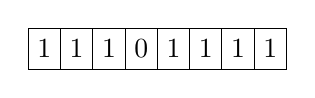
\begin{tikzpicture}[every node/.style={block},
        block/.style={minimum height=1.5em,outer sep=0pt,draw,rectangle,node distance=0pt}]
   \node (A) {1};
   \node (B) [right=of A] {1};
   \node (C) [right=of B] {1};
   \node (D) [right=of C] {0};
   \node (E) [right=of D] {1};
   \node (F) [right=of E] {1};
   \node (G) [right=of F] {1};
   \node (H) [right=of G] {1};
\end{tikzpicture}
\end{center}
We can always assume that the input tape will have the correct formatting and that the Turing machine will always start at the leftmost '1' of the tape. All we need to do is move the left most '1' in between the two numbers and then remove an extra '1' at the beginning. We can represent this process with the following graph.

\begin{center}
\begin{tikzpicture}[scale=0.2]
\tikzstyle{every node}+=[inner sep=0pt]
\draw [black] (3.3,-9.3) circle (3);
\draw (3.3,-9.3) node {$s_0$};
\draw [black] (21.8,-9.3) circle (3);
\draw (21.8,-9.3) node {$s_1$};
\draw [black] (38.8,-9.3) circle (3);
\draw (38.8,-9.3) node {$s_2$};
\draw [black] (59.3,-9.3) circle (3);
\draw (59.3,-9.3) node {$s_3$};
\draw [black] (59.3,-24.3) circle (3);
\draw (59.3,-24.3) node {$HALT$};
\draw [black] (6.3,-9.3) -- (18.8,-9.3);
\fill [black] (18.8,-9.3) -- (18,-8.8) -- (18,-9.8);
\draw (12.55,-8.8) node [above] {$1\rightarrow0,R$};
\draw [black] (24.8,-9.3) -- (35.8,-9.3);
\fill [black] (35.8,-9.3) -- (35,-8.8) -- (35,-9.8);
\draw (30.3,-8.8) node [above] {$0\rightarrow1,L$};
\draw [black] (41.8,-9.3) -- (56.3,-9.3);
\fill [black] (56.3,-9.3) -- (55.5,-8.8) -- (55.5,-9.8);
\draw (49.05,-8.8) node [above] {$0\rightarrow0,R$};
\draw [black] (20.477,-6.62) arc (234:-54:2.25);
\draw (21.8,-2.05) node [above] {$1\rightarrow1,R$};
\fill [black] (23.12,-6.62) -- (24,-6.27) -- (23.19,-5.68);
\draw [black] (37.9,-6.45) arc (225.25384:-62.74616:2.25);
\draw (41.13,-1.81) node [above] {$1\rightarrow1,L$};
\fill [black] (40.51,-6.85) -- (41.43,-6.64) -- (40.72,-5.93);
\draw [black] (59.3,-12.3) -- (59.3,-21.3);
\fill [black] (59.3,-21.3) -- (59.8,-20.5) -- (58.8,-20.5);
\draw (59.8,-16.8) node [right] {$1\rightarrow0,R$};
\draw [black] (3.3,-16.1) -- (3.3,-12.3);
\fill [black] (3.3,-12.3) -- (2.8,-13.1) -- (3.8,-13.1);
\end{tikzpicture}
\end{center}

\end{ex}


\subsection{Multitape Turing Machine}
Turing machines do not necessarily only have to have a single tape. Turing machines can be constructed such that they can have any number of tapes at the same time. Each tape in a multitape Turing machine act independently from each other and their contents do not mix, they also have independent tape heads. 
\begin{defn}
The definition of a multitape Turing machine is the same as a regular one except for the transition function as it is now defined as 
\begin{itemize}
\item $\delta$: $Q \times \Gamma^k \rightarrow Q \times (\Gamma \times (RL))^k$
\end{itemize}
such that $k$ is the number of tapes the Turing machine has.
\end{defn} \cite{siu}

An example of a three tape Turing machine can be shown below.
\begin{center}
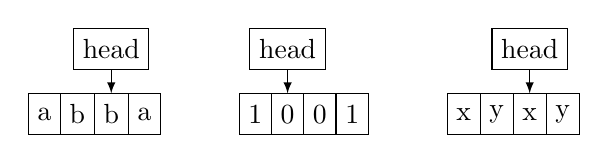
\begin{tikzpicture}[every node/.style={block},
        block/.style={minimum height=1.5em,outer sep=0pt,draw,rectangle,node distance=0pt}]
   \node (A) {a};
   \node (B) [right=of A] {b};
   \node (C) [right=of B] {b};
   \node (D) [right=of C] {a};
   \node (F) [above = 0.3cm of C] {head};
   \draw[-latex] (F) -- (C);
   
   \node (G) [right = 1 cm of D] {1};
   \node (H) [right=of G] {0};
   \node (I) [right=of H] {0};
   \node (J) [right=of I] {1};
   \node (K) [above = 0.3cm of H] {head};
   \draw[-latex] (K) -- (H);
      
   \node (V) [right = 1 cm of J] {x};
   \node (X) [right=of V] {y};
   \node (Y) [right=of X] {x};
   \node (Z) [right=of Y] {y};
   \node (AA) [above = 0.3 cm of Y)] {head};
   \draw[-latex] (AA) -- (Y);
\end{tikzpicture}
\end{center}
From left to right, let us label each tape 1,2 and 3. If we are to draw out a multitape Turing machine in a graph as we have done before, we need to change our formatting slightly. Assume we want to create a transition that does the following for each tape:\\
\textbf{tape 1) } if 'b' is read, write 'a' and move right\\
\textbf{tape 2) } if '0' is read, write '0' and move right\\
\textbf{tape 3) } if 'x' is read, write 'y' and move left\\
We can then represent our transitions as such
\[ b0x \rightarrow a0y, RRL \]
where for each section of the transitions, the leftmost character represents the first tape.
\begin{thm}
Every multitape Turing machine can be reconstructed as a single-tape Turing machine.
\end{thm}
\begin{proof}
We have some input string represented as $w_1w_2 \cdots w_n$ where $n$ is the length of the string. We then place all the separate tapes onto a single tape and add a dot on top of each symbol where the tape head resides for each tape, divide the tapes by using a '$\#$'. 
\[ \#\dot{w_1}w_2 \cdots w_n \# \dot{\sqcup} \# \dot{\sqcup} \# \cdots \# \]
Once we have created the single tape, we scan through the entire tape to find all the heads, then re-run through the entire tape to following the instructions of the original multitape Turing machine. If during the process one of the 'tape heads' reaches a $\#$, then shift the entire tape and add in a blank symbol.
\end{proof}
From this process, let us take the three tapes we had and convert it into a single tape
\begin{center}
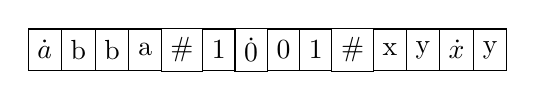
\begin{tikzpicture}[every node/.style={block},
        block/.style={minimum height=1.5em,outer sep=0pt,draw,rectangle,node distance=0pt}]
   \node (A) {$\dot{a}$};
   \node (B) [right=of A] {b};
   \node (C) [right=of B] {b};
   \node (D) [right=of C] {a};
   \node (E) [right=of D] {$\#$};    
   \node (F) [right=of E] {1};
   \node (G) [right=of F] {$\dot{0}$};
   \node (H) [right=of G] {0};
   \node (I) [right=of H] {1};      
	 \node (J) [right=of I] {$\#$};   
   \node (K) [right=of J] {x};
   \node (L) [right=of K] {y};
   \node (M) [right=of L] {$\dot{x}$};
   \node (N) [right=of M] {y};

\end{tikzpicture}
\end{center}
Note that although all multitape Turing machines can be converted into a single tape Turing machine, it increases the runtime making the process much slower.


\subsection{Non-deterministic Turing Machines}
Similar to DFA's and NFA's, Turing machines can also be constructed to be non deterministic.
\begin{defn}
The definition of a non-deterministic Turing machine is the same except for the transition function which we now define as 
\begin{itemize}
\item $\delta: Q \times \Sigma \rightarrow P \{ \Gamma \times (RL) \times Q \}$
\end{itemize}
Where $P$ represents the power set, to account for all the different branches possible in a non-deterministic machine
\end{defn} \cite{eric}

As an example, let us look at this graph of a non-deterministic Turing machine.
\begin{center}
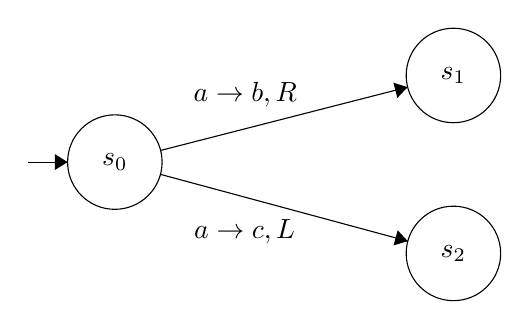
\begin{tikzpicture}[scale=0.2]
\tikzstyle{every node}+=[inner sep=0pt]
\draw [black] (5.7,-8.7) circle (3);
\draw (5.7,-8.7) node {$s_0$};
\draw [black] (27.2,-3.2) circle (3);
\draw (27.2,-3.2) node {$s_1$};
\draw [black] (27.2,-14.5) circle (3);
\draw (27.2,-14.5) node {$s_2$};
\draw [black] (8.61,-7.96) -- (24.29,-3.94);
\fill [black] (24.29,-3.94) -- (23.39,-3.66) -- (23.64,-4.63);
\draw (13.98,-5.22) node [above] {$a\rightarrow b,R$};
\draw [black] (0.2,-8.7) -- (2.7,-8.7);
\fill [black] (2.7,-8.7) -- (1.9,-8.2) -- (1.9,-9.2);
\draw [black] (8.6,-9.48) -- (24.3,-13.72);
\fill [black] (24.3,-13.72) -- (23.66,-13.03) -- (23.4,-13.99);
\draw (13.94,-12.3) node [below] {$a\rightarrow c,L$};
\end{tikzpicture}
\end{center}
Let us have some input tape as such, where to dotted symbol indicates the location of the tape head.
\begin{center}
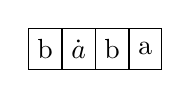
\begin{tikzpicture}[every node/.style={block},
        block/.style={minimum height=1.5em,outer sep=0pt,draw,rectangle,node distance=0pt}]
   \node (A) {b};
   \node (B) [right=of A] {$\dot{a}$};
   \node (C) [right=of B] {b};
   \node (D) [right=of C] {a};
\end{tikzpicture}
\end{center}
Similar to NFA's, since the state $s_0$ has two possibilities, we have to consider both possible branches. Now, we have two different tapes to account for
\begin{center}
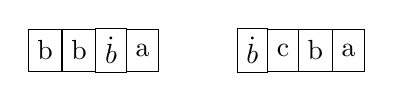
\begin{tikzpicture}[every node/.style={block},
        block/.style={minimum height=1.5em,outer sep=0pt,draw,rectangle,node distance=0pt}]
   \node (A) {b};
   \node (B) [right=of A] {b};
   \node (C) [right=of B] {$\dot{b}$};
   \node (D) [right=of C] {a};
   
   \node (E) [right= 1 cm of D] {$\dot{b}$};
   \node (F) [right=of E] {c};
   \node (G) [right=of F] {b};
   \node (H) [right=of G] {a};
\end{tikzpicture}
\end{center}
When a branch of the Turing machine calculations halt and accept the string, then the Turing machine accepts the string. However, in order for the Turing machine to reject, all branches have to either reject or die out(tape ends in a non final state). If a branch never halts, then we count that has the branch dying out.

\begin{thm}
Every non-deterministic Turing machine has an equivalent deterministic Turing machine that accepts the same language
\end{thm}

We understand that when running a non-deterministic Turing machine, we have to account for all branches. However, since it is impossible to tell which branch will make the Turing machine halt, we need to simulate all of them. Since non-deterministic automata in general have to consistently branch out, we can create a tree of all the possible 'decisions' that the Turing machine makes. Lets take an arbitrary tree to use in our example.
\begin{center}
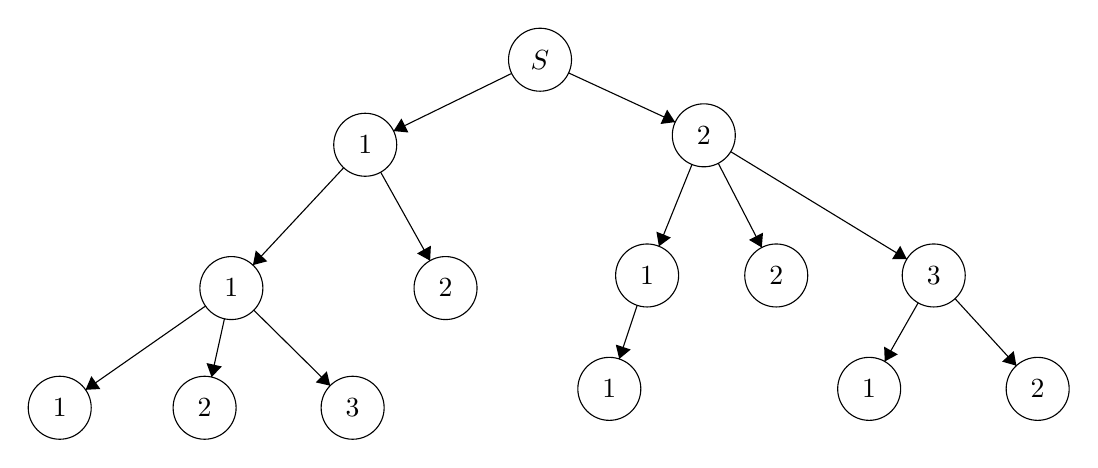
\begin{tikzpicture}[scale=0.2]
\tikzstyle{every node}+=[inner sep=0pt]
\draw [black] (32.8,-2.2) circle (2);
\draw (32.8,-2.2) node {$S$};
\draw [black] (21.7,-7.6) circle (2);
\draw (21.7,-7.6) node {$1$};
\draw [black] (43.2,-7) circle (2);
\draw (43.2,-7) node {$2$};
\draw [black] (13.2,-16.7) circle (2);
\draw (13.2,-16.7) node {$1$};
\draw [black] (26.8,-16.7) circle (2);
\draw (26.8,-16.7) node {$2$};
\draw [black] (39.6,-15.9) circle (2);
\draw (39.6,-15.9) node {$1$};
\draw [black] (47.8,-15.9) circle (2);
\draw (47.8,-15.9) node {$2$};
\draw [black] (57.8,-15.9) circle (2);
\draw (57.8,-15.9) node {$3$};
\draw [black] (37.2,-23.1) circle (2);
\draw (37.2,-23.1) node {$1$};
\draw [black] (53.7,-23.1) circle (2);
\draw (53.7,-23.1) node {$1$};
\draw [black] (64.4,-23.1) circle (2);
\draw (64.4,-23.1) node {$2$};
\draw [black] (2.3,-24.3) circle (2);
\draw (2.3,-24.3) node {$1$};
\draw [black] (20.9,-24.3) circle (2);
\draw (20.9,-24.3) node {$3$};
\draw [black] (11.5,-24.3) circle (2);
\draw (11.5,-24.3) node {$2$};
\draw [black] (31,-3.07) -- (23.5,-6.73);
\fill [black] (23.5,-6.73) -- (24.44,-6.82) -- (24,-5.93);
\draw [black] (34.62,-3.04) -- (41.38,-6.16);
\fill [black] (41.38,-6.16) -- (40.87,-5.37) -- (40.45,-6.28);
\draw [black] (20.33,-9.06) -- (14.57,-15.24);
\fill [black] (14.57,-15.24) -- (15.48,-15) -- (14.75,-14.31);
\draw [black] (22.68,-9.34) -- (25.82,-14.96);
\fill [black] (25.82,-14.96) -- (25.87,-14.01) -- (24.99,-14.5);
\draw [black] (42.45,-8.85) -- (40.35,-14.05);
\fill [black] (40.35,-14.05) -- (41.11,-13.49) -- (40.19,-13.12);
\draw [black] (44.12,-8.78) -- (46.88,-14.12);
\fill [black] (46.88,-14.12) -- (46.96,-13.18) -- (46.07,-13.64);
\draw [black] (44.91,-8.04) -- (56.09,-14.86);
\fill [black] (56.09,-14.86) -- (55.67,-14.02) -- (55.15,-14.87);
\draw [black] (38.97,-17.8) -- (37.83,-21.2);
\fill [black] (37.83,-21.2) -- (38.56,-20.6) -- (37.61,-20.29);
\draw [black] (56.81,-17.64) -- (54.69,-21.36);
\fill [black] (54.69,-21.36) -- (55.52,-20.91) -- (54.65,-20.42);
\draw [black] (59.15,-17.37) -- (63.05,-21.63);
\fill [black] (63.05,-21.63) -- (62.88,-20.7) -- (62.14,-21.37);
\draw [black] (12.76,-18.65) -- (11.94,-22.35);
\fill [black] (11.94,-22.35) -- (12.6,-21.68) -- (11.62,-21.46);
\draw [black] (14.62,-18.1) -- (19.48,-22.9);
\fill [black] (19.48,-22.9) -- (19.26,-21.98) -- (18.56,-22.69);
\draw [black] (11.56,-17.84) -- (3.94,-23.16);
\fill [black] (3.94,-23.16) -- (4.88,-23.11) -- (4.31,-22.29);
\end{tikzpicture}
\end{center}

Where $S$ is that start and the numbers simply represent the possible choices when we reach a non-deterministic situation. For instance, a path that we simulate may be represented as "231". With all the possible paths in mind, we can construct out deterministic Turing machine, specifically a multitape Turing machine. This machine will have three separate tapes which do the following:
\begin{itemize}
\item \textbf{Tape 1:} This tape is the input tape, this tape is never modified and simply read from.
\item \textbf{Tape 2:} The 'main' tape, where the simulation of a regular single tape Turing machine occurs. This tape is empty during the start of the process.
\item \textbf{Tape 3:} Contains all the possible paths within the tree.
\end{itemize}
With these three tapes, our process looks like this:
\begin{enumerate}
\item Copy the contents from tape 1 to tape 2
\item Consult tape 3 as to which 'path' on the tree to take
\item Use tape 2 to simulate the path stored in tape 3
\item Increment onto the next path in tape 3
\item reset tape 2 and repeat the whole process
\end{enumerate}
Throughout the process, if one of the branches leads to the Turing machine accepting the branch, then we can halt early and accept. Otherwise, we keep simulating all the branches and eventually reject if nothing is accepted.


\subsection{Turing Machines and Languages}
Here are some terminology of Turing machines and languages \cite{kozen}
\begin{defn}
Let there be a language $L$ and a Turing machine $T$. If the machine $T$ accepts all strings in $L$ and rejects all strings that do not exist within $L$. i.e. the Turing machine T will always halt, no matter the input. Then tha language $L$ is known as a \textbf{recursive language}
\end{defn}

\begin{defn}
Let there be a language $L$ and a Turing machine $T$. If $T$ accepts and halts on all strings in $L$, but may not necessarily halt for strings not in $L$. Then the language $L$ is known as \textbf{recursively enumerable language}
\end{defn}

If a language $L$ is either recursive or recursively enumerable on a Turing machine $T$. Then we can say that $T$ recognizes the language $L$.

\begin{defn}
If a language $L$ is a recursive language, then $L$ is known as a \textbf{decidable language}. Note that the reverse of this statement is also true.
\end{defn}

\begin{defn}
A language $L$ is a recursively enumerable language, then it is also known as a \textbf{partially decidable language}. The reverse is also true.
\end{defn}

\begin{defn}
A language $L$ is \textbf{undecidable} if it is not a deciable language. This means that it is possible for an undeciable language to be partially decidable. If the language is not partially decidable, then there exists no Turing machine that exists to accept $L$.
\end{defn}


\section{The Halting Problem}
We understand that Turing machines can either halt, accept or reject, or never halt from being stuck in an infinite loop within its program. The halting problem asks a very simple questions. For some Turing machine $T$ and an input $i$, can we build a Turing machine that will always tell us if $T$ will halt or never halt, given the input $i$?\cite{salvador}\\  

Formally, we can define the halting problem as a language $H$. Such that $H$ is the set of all inputs $<T,i>$ such that $T$ is a Turing machine and halts on the input $i$. If there exists some other Turing machine $M$ such that for all $(T, i) \in H$, $M$ will halt and accept the input, then we have solved the halting problem. However, the halting problem has been proven the be \textbf{undecidable} and thus, unsolvable.


\subsection{Properties of the Halting Problem}

We can show that the halting problem is undecidable through a proof by contradiction.
\begin{proof}
Assume that we have some Turing machine $M$ that perfectly solves the halting problem. So given two inputs, some Turing machine $T$ and and input $i$. If we were to give both inputs of $M$ as itself, then $M$ should halt and accept.\\

Now let us create a new Turing machine $M'$. $M'$ will depend on $M$, as if $M$ determines that the given inputs will halt, then $M'$ will reject and not halt. If $M$ rejects the input and doesn't halt, then $M'$ will halt. Now, if the inputs of $M'$ are $M'$ itself, we have two cases:
\begin{itemize}
\item if $M$ accepts the input and deems that $M'$ will halt. However, by definition of $M'$, it will never halt.
\item if $M$ deems that $M'$ will never halt. Then by definition of $M'$ it will halt
\end{itemize}
In either case, we have a contradiction. Since we had made the assumption that $M$ will always give us the correct output given its inputs, $M'$ shows us that a Turing machine $M$ can not exist, and thus the halting problem is undecidable.
\end{proof}

However, we can show that the halting problem is \textbf{recognizable}.
\begin{proof}
Recall that a language $L$ is recognizable if there exists a machine that accepts all inputs in $L$ and either rejects, or never halts in strings not in $L$. In the case of inputs in $H$, we can simply use a universal Turing machine $U$. If the machine $U$ takes inputs $<T,i> \in H$, then by definition, $U$ will accept if $T$ accepts $i$, and reject or never halt if $T$ does so. Then this shows that $H$ is a recognizable language.
\end{proof}


\subsection{Applications of the Halting Problem}
Despite the halting problem being unsolvable by computational means, it does not mean we have not learned anything from it. The main benefit mathematicians and computer scientist learned from the halting problem is the fact it is proven to be undecidable. From this, the halting problem has been used to prove other undecidable problems.\\

If we are able to reduce a problem to the halting problem, then it is immediately proven to be undecidable. This could be done by simply showing that the problem is the same, or formulating a proof similar in style to the halting problem.\cite{wood} \\
Hypothetically, if the halting problem were solvable, it would be possible to solve some unsolved problems, these include the following:
\begin{itemize}
\item \textbf{Goldbach Conjecture}: ever even counting number greater than 2 is equal to the sum of two primes. \cite{gold}
\item \textbf{Kolomgorov Complexity}: The smallest amount of computing power needed to produce an object
\item \textbf{The Collatz Conjecture}: More famously known as the $3n + 1$ problem\cite{simon}
\end{itemize}
If the halting problem was solvable, and there did exist a Turing machine that could solve it, then we could also construct one that could solve all of the above problems. However, since it is not possible, these problems have to remain unsolved for the time being.



\subsection{Rice's Theorem}
From the proof of the halting problem, Rice's theorem was developed to generalize all undecidable problems that were reducable to the halting problem.
\begin{defn}
Let $P$ be some non-trivial property of a language, and the language that has said property, we label as $L_p$. If the language is recognized by some Turing machine $T$ then we say
\[ L_p = \{ <T> | L(M) \in P \} \]
is undecidable
\end{defn}
Note that $P$ is merely a set of languages. If $L \in P$ then we say that $L$ satisfies the property $P$. $P$ is also called trivial if it is satisfied by all recursively enumerable languages, or it is no satisfied by any at all. \cite{bulma}


\subsection{Orcale machines}
From the study of decision problems such as the halting problem, in complexity and computability theory, there cam about another abstract machine called an oracle machines. These machines can be thought of as a Turing machine with an \textbf{oracle} connected to them. These oracles are essentially black boxes that can solve decision problems. These machines are purely theoretical.\\

The definition of an oracle machine is similar to that of a Turing machine. However, in addition an oracle machine adds the following components:
\begin{itemize}
\item \textbf{Oracle tape}: a separate tape from the Turing machine, and has a different alphabet.
\item \textbf{Oracle head}: similar to the tape head of a Turing machine, but purely meant for the oracle tape
\item \textbf{States}: Two special states are added, the ASK and RESPONSE state.
\end{itemize}
Now, an oracle machine can solve the original halting problem of just regular Turing machines, since it can decide if a Turing machine will halt or not. However, we essentially have another halting problem with oracle machines itself as it is unable to tell if machines such as itself will halt or not. This can be proven in the same way we did with the original problem.
\begin{thebibliography}{book}

 

\bibitem{Aora} Arora, Neeraj. (2018). Introduction to Turing Machine. 

\bibitem{brod} Brodkorb, Laurel. The Entscheidungsproblem and Alan Turing - Georgia College \& State https://www.gcsu.edu/sites/files/page-assets/node-808/attachments/brodkorb.pdf. 

\bibitem{bulma} Bulma. “CSC 341 (Fall 2021).” Rice's Theorem, https://osera.cs.grinnell.edu/csc341/readings/rices-theorem.html. 

\bibitem{Chris} Brown, Christopher W. SI340: Functions \& a Formal Definition of a DFA, https://www.usna.edu/Users/cs/wcbrown/courses/F17SI340/lec/l05/lec.html. 

\bibitem{Ben} Chor, Benny. A Deterministic FInite Automaton (DFA) Is a 5-Tuple. https://www.cs.tau.ac.il/~bchor/CM/Compute2-Printer.pdf. 

\bibitem{stan}De Mol, Liesbeth. “Turing Machines.” Stanford Encyclopedia of Philosophy, Stanford University, 24 Sept. 2018, https://plato.stanford.edu/entries/turing-machine/text=Turing\%20machines\%2C\%20first\%20described\%20by,the\%20computing\%20of\%20real\%20numbers. 

\bibitem{eric} Erickson, Jeff. “Lecture 38: Nondeterministic Turing Machines.” 

\bibitem{gao} Gao, Alice. Alice Gao's CS 245 Resources Page, https://cs.uwaterloo.ca/~a23gao/cs245-s18/index.shtml. 

\bibitem{gold} “Goldbach Conjecture.” Encyclopædia Britannica, Encyclopædia Britannica, Inc., https://www.britannica.com/science/Goldbach-conjecture.

\bibitem{hehner} Hehner, Eric. Problems with the Halting Problem - Department of Computer Science ... https://www.cs.toronto.edu/~hehner/PHP.pdf. 

\bibitem{john} John E. Hopcroft and Rajeev Motwani and Jeffrey D. Ullman (2003). Introduction to Automata Theory, Languages, and Computation

\bibitem{kam} Kamvysselis, Manolis. Universal Turing Machine, https://web.mit.edu/manoli/turing/www/turing.html. 

\bibitem{kozen} Kozen, D.C. (1997), Automata and Computability



\bibitem{simon} Letherman, Simon, et al. The 3n+1 Problem and Holomorphic Dynamics. A K Peters, Ltd. 

\bibitem{salvador} Salvador Lucas,The origins of the halting problem,Journal of Logical and Algebraic Methods in Programming,Volume 121,2021,100687,ISSN 2352-2208,https://doi.org/10.1016/j.jlamp.2021.100687.(https://www.sciencedirect.com/science/article/pii/S235222082100050X)



\bibitem{Turing} Turing, Alan. On Computable Numbers, with an Application to Computer Science. https://www.cs.virginia.edu/robins/TuringPaper1936.pdf. 


\bibitem{siu} Siu, Christopher. “Multitape Turing Machines.” Christopher Siu, http://users.csc.calpoly.edu/~cesiu/. 

\bibitem{wood} Wood, Ben. “Computability and the Halting Problem.” CS 251: Computability and the Halting Problem, https://cs.wellesley.edu/~cs251/s21/notes/halt.html. 

\bibitem{robert} Robertson, Benjamin W. CSCE-433-500/CSCE-627-600 (Spring 2022), https://people.engr.tamu.edu/j-chen3/courses/627/2022/courseweb.html. 

\end{thebibliography}

\end{document} 






